\documentclass[12pt,english]{article}
\usepackage[utf8]{inputenc}
\usepackage{tgpagella} % Palatino text only
\usepackage{mathpazo}  % Palatino math & text
\usepackage[left=1.5in,right=1.5in,top=1.5in,bottom=1.5in]{geometry}
% \linespread{1.5}
% \usepackage[super,comma,sort]{natbib}
\usepackage{bibunits} % To get multiple bibliography
\usepackage[round,sort&compress]{natbib}
\usepackage{url} % [hyphens]
\usepackage[hyperpageref]{backref} % back references biblio. Needs latexmk at compilation.
\usepackage[pagebackref]{hyperref}
% Lines below required to make pagebackref compatible with bibunits
\usepackage{etoolbox}
\makeatletter
\patchcmd\Hy@backout{\@auxout}{\@mainaux}{}{\fail}
\patchcmd\Hy@backout{\@auxout}{\@mainaux}{}{\fail} %yes twice the same line
\makeatother
% \usepackage{multibib} % incompatible with backref
\hypersetup{
  colorlinks=true, % breaklinks=true,
  urlcolor=purple,    % color of external links
  linkcolor=blue,  % color of toc, list of figs etc.
  citecolor=violet,   % color of links to bibliography
}
\usepackage{bm}
\usepackage{indentfirst}
\usepackage{tocbibind}
\setcitestyle{aysep={}} 
\usepackage{amsmath}
\usepackage{amssymb}
\usepackage{eurosym}
\usepackage{amsfonts}
\usepackage{enumerate}
\usepackage{babel}
\usepackage{caption}
\usepackage{supertabular}
\usepackage{tabularx}
\usepackage{float}
\usepackage{dsfont}
\usepackage{fancyvrb}
\usepackage{verbatim}
\usepackage{enumitem}
\usepackage{setspace}
\usepackage{comment}
\usepackage{subcaption}
\usepackage{graphicx}
\usepackage{tikz}
\usepackage{gensymb}
\usepackage{textcomp}
\usepackage{bibentry} % to use nobibliography

\usepackage{tabulary}
\usepackage{tabularx}
\usepackage{booktabs}
\usepackage{fullpage}
\usepackage{morefloats}
\usepackage{makecell}
\usepackage{lscape}
\usepackage{pdflscape}
\usepackage{longtable}
\usepackage{rotating}
\usepackage{xcolor}% header
\usepackage{titlesec} % To change size of Bibliography heading
\usepackage{fancyhdr}

% Header on every page except frontpage (handled by tikz)
% \pagestyle{fancy}% header
% \renewcommand{\headrulewidth}{0pt} % removes horizontal line from header
% \setlength{\headheight}{62pt} % adjust the nb of pt here and below if there is a warning
% \addtolength{\topmargin}{-62pt}
% \fancyhead[R]{} % removes section title from header
% \fancyhead[L]{} % removes section title from header
% \chead{\href{http://global-redistribution-advocates.org}{
\includegraphics[height=1cm]{../figures/policies/logo_full_white_bg}}\\ \quad }

\usepackage{tocloft}
\usepackage{titletoc}
\usepackage{csquotes}
\usepackage{tcolorbox}
\usepackage[export]{adjustbox}
\usepackage[anythingbreaks]{breakurl} % for links
\usepackage{multicol}
\usepackage{lineno}
\linenumbers

\usepackage{abstract}
\addto\captionsenglish{\renewcommand{\abstractname}{}}    % clear the title
\renewcommand{\absnamepos}{empty} % originally center
\newsavebox\ltmcbox % For net gain table over two columns
%\usepackage[nomarkers,figuresonly]{endfloat} % Figures at the end
%\usepackage[section,below]{placeins} % Floats placed in the section they appear in.
\renewcommand{\floatpagefraction}{.9}

\title{An International Plan for Sustainable Development
%\textit{A shared vision towards global climate justice}
} 
\defaultbibliographystyle{plainnaturl_clean}
\defaultbibliography{global_tax_attitudes}

% \author{Adrien Fabre,\footnote{Corresponding author. CNRS; Paris, 75016, France and CIRED, Nogent-sur-Marne, 94130, France. Email: adrien.fabre@cnrs.fr.} \;
% Rabah Arezki,\footnote{CNRS, Paris, 75016, France and Harvard’s Kennedy School of Government, Cambridge, 02138, USA.} \;
% Dipak Dasgupta,\footnote{The Energy and Resources Institute, New Delhi, 110003, India.} \;
% Bin Hu,\footnote{Institute of Climate Change and Sustainable Development, Tsinghua University, Beijing, 100190, China.}  \\
% Partha Sen,\footnote{Centre for Development Economics, Delhi School of Economics, Delhi, 110007, India and CESifo, Munich, 81679, Germany.}  \;
% Frederick van der Ploeg\footnote{Department of Economics, University of Oxford, Oxford, OX1 3UQ, UK, University of Amsterdam, the Netherlands, and CEPR.} }
%\footnote{CNRS researcher in economics at CIRED. E-mail: adrien.fabre@cnrs.fr.}
% } 
% \author{Global Redistribution Advocates\footnote{The author is Adrien Fabre, CNRS researcher in economics at CIRED. E-mail: adrien.fabre@cnrs.fr.}} 

% TODO? Ideas from Andreas Bummel. Reduce the endorsement threshold 1M => 500k. Cut the budget (no staffers, 30M per list). Widen the mandate (though not a condition for DwB support): say the assembly would primarily work on climate but could propose things on any domain.

\date{\today{} %-- \href{https://github.com/bixiou/global_tax_attitudes/raw/main/paper/policy_brief_taxes.pdf}{Link to most recent version}
} 

\begin{document}

\maketitle
% \tikz [remember picture, overlay] %
% \node [shift={(5.5cm,-1.5cm)}] at (current page.north west) % north west
% [anchor=north west] % north west
% {\href{http://global-redistribution-advocates.org}{
\includegraphics[height=1.3cm]{../figures/policies/logo_full_white_bg}}};

\clearpage
\begin{abstract}
  Renewed momentum to combat climate change and global poverty can be achieved by embracing a shared vision on international carbon pricing and new global taxes, with proper allocation of revenues and conditional cooperation mechanisms. We put forward a sketch of a treaty that sets up new taxes on wealth, polluting fuels, financial transactions, and corporate income, raising more than \$3 trillion per year. Part of the revenue from these taxes would finance international transfers. One percent of each countr's GNI would be reallocated to each country in proportion to their population, which would address climate finance needs and foster sustainable development. According to recent surveys, this vision for sustainable development is supported by majorities worldwide.
\end{abstract}

\textbf{Keywords}: Climate policy; carbon price; SDGs; poverty; international taxation.

\textbf{JEL}: Q56; F38; H23; Q54; H87; F64; Q58; F53; F35.

\onehalfspacing
\renewcommand\bibname{References} 
\begin{bibunit}

% \clearpage

\section{Introduction}
After years of slow progress, international negotiations on climate and taxation issues have yet to deliver ambitious agreements that secure decarbonization, clamp down on tax evasion, and foster international cohesion. We therefore suggest the contours of a fair agreement between voluntary countries aimed to ensure climate neutrality and sustainable development. We believe that our proposal will be supported by a majority of citizens worldwide.
A broad set of countries currently are actively cooperating to develop a transformative agenda for all the people on the planet, including a new UN Framework Convention on International Tax Cooperation (UNFCITC), and an expansion of the lending headroom of Multilateral Development Banks (MDBs) by \$400 billion. Recent successes ought to be reproduced on neighboring issues.

We seek a plan that meets the following criteria: it must achieve the Paris agreement temperature target; meet the Sustainable Development Goals; be efficient; and be acceptable by most countries and people. While plans for climate action or international tax justice have already been proposed \citep{pisani-ferry_global_2025,zucman_blueprint_2024,bolton_why_2025}, they often fail to meet all our criteria. Our ambition is to offer a shared vision to address climate change and global poverty, which translates into commonly agreed principles and instruments.

An International Sustainable Union for Climate and Redistribution
While decisions at the UNFCCC require unanimity, a subset of countries can begin to work productively to propose ambitious agreements, with no need for universal participation, on the condition that they are fair and open to all countries.

We stress the necessity of an equitable climate outcome and acknowledge the responsibility of developed countries, whose current income level stems from a historical accumulation of capital that benefited from their past emissions. Meanwhile, it is time to move beyond the simple dichotomy between developing and developed countries as, compared to 30 years ago, some countries are no longer developing countries. For example, Slovenia, South Korea, Saudi Arabia, and Singapore are classified with developing countries by the UNFCCC though they are richer than Greece, which is considered a developed country. We prefer simple yet continuous, harmonized and up-to-date measure of development, such as GNI per capita, as basis for countries' contributions and entitlements. This is already used as the basis of a range of international arrangements from eligibility to International Development Association loan terms to allocation of Special Drawing Rights. As a benchmark (from which some adjustments can be made to account for specific cases), we suggest that contributions should be proportional to a country's GNI while transfers should be proportional to the size of its population. Of course, one could do more by asking developed countries that have emitted more since the beginning of the Industrial Revolution to contribute more but it would be less politically feasible.

We need to act now as any delay comes with deadly costs, disproportionately borne by low-income countries. Furthermore, such delays come with further distortions as they provoke fossil fuel producers to boost extraction while the going is good (the so-called ``Green Paradox''). Ensuring flows of, and access to, adequate climate finance is key to the implementation and delivery of the Paris Agreement, as well as to achieving the transition required to address the climate crisis. Developed countries should fulfill their financial commitments set out in the UNFCCC and Paris Agreement. We believe that it is in their best interest to go much further \citep{bolton_why_2025}. Only by providing adequate financial conditions to developing countries can we address climate change and avoid its daunting costs.

Climate change requires responses of three types: mitigation, adaptation, and funding of losses and damages. Climate finance should be broken down into these three types too. Although market loans from the private sector play a major role in mitigation and adaptation, they play no role in funding losses and damages. Soft loans from development banks play a capital-heavy role in adaptation, but less so for mitigation and not at all for losses and damages. Furthermore, grants from donors play a critical role in losses and damages. The policy responses should thus be tailored to the specific response type. For mitigation, one key element is to address capital market imperfections and lower the cost of capital in the Global South through multilateral guarantees. Adaptation is largely addressed by the recapitalization of MDBs. Lastly, increased grants are needed for adaptation and losses and damages.

The high cost of capital in developing countries remains a great challenge for mitigation and adaptation. Public finance is an indispensable lever for private finance to swiftly mobilize private sector investment on a large scale. Public guarantees and soft loans are needed to protect investors from foreign exchange and sovereign risks \citep{hourcade_climate_2025}.

Beyond making low-carbon investments more profitable, we must also shift the current system away from fossil fuels. We should make polluters pay and progressively develop the international pricing of greenhouse gas emissions. Representative surveys from 20 countries show very strong support for climate policies that are at the global level. These surveys indicate the presence of strong majority support for a global carbon price and a consensus in favor of an equal per capita allocation of its revenue \citep{fabre_majority_2025}.

While previous attempts of international carbon pricing have failed, this time may be different for three reasons. First, we now know that the public at large supports a global carbon price. Second, the world population shares a common norm on how to share the revenues from a global carbon price: the equal per capita allocation. Third, rather than seeking universal agreement among all countries, a Sustainable Union can be formed by a broad set of ambitious countries (a coalition of the willing).

\section{Carbon Pricing}
In the short term, countries participating in the Sustainable Union would establish a carbon price floor of \$10 per ton of CO$_\text{2}$. This floor roughly corresponds to the carbon price on China's national carbon market. A share of the carbon price revenues raised in any country would be pooled at the international level and rebated to participating countries in proportion to their population size. The pooled amount would be proportional to the country's GNI, which ensures that transfers take place from rich to poor countries. The more GNI per capita of a country exceeds the world average, the more a country contributes. Countries with a GNI per capita below the world average benefit from the pooling and rebating of carbon price revenues. In the medium term, the Union would establish an international competitive market for carbon permits. Once the carbon market is fully in place, the Union would auction emission permits to fossil fuel companies upstream. The permit quota would be reduced each year, until it reaches zero at a predetermined date, say 2075. The quota would respect a global emissions target compatible with the objectives of the Paris Agreement. To leave a fair carbon budget to countries outside the Union, the quota would correspond to the emissions target scaled by the Union's share of the world's population.
The carbon market does not imply a uniform carbon price, because some countries may choose to implement a higher carbon price than the international one. To avoid carbon leakage resulting from differentiated carbon prices, carbon border tax adjustments are needed. However, such adjustments should be coordinated, and their implementation overseen by a multilateral institution to assess tax liabilities and arbitrate disputes impartially. Besides, participating countries would commit either not to tax the carbon content of imports from one another or to return the tax collected to the exporting country if they do so. This would neutralize the carbon tariff for participating countries. More than in the details of carbon tariffs, high stakes lie in the allocation of the carbon market's emissions rights.

As a benchmark, each country would be granted emissions rights proportional to its population. There would be some adjustments to the benchmark, in line with specific needs and ambition of certain regions (see Table \ref{tab:budgets}). In particular, China and the EU would receive emissions rights corresponding to their own, ambitious decarbonization pathway. Importantly, integrating all countries' emissions within a common market guarantees that each country respects its target. For example, if the EU ends up emitting more than it aimed for, this will be compensated by other countries (e.g. in Africa) emitting less than the world average and selling unused emissions rights to the EU. Emissions reductions will take place where they are the least costly, ensuring efficiency. To the extent that the price of carbon is higher than the price floor, additional transfers will flow from rich to poor countries, spurring much needed growth and poverty reduction in lower-income countries. 

\begin{table}[h]
  \caption{Carbon budget over 2030-2080 (in GtCO$_\text{2}$): budgets proposed and equal per capita budgets.\label{tab:budgets}} 
  \makebox[\textwidth][c]{
\begin{tabular}[t]{ccccccccc}
  \toprule 
   & Africa & China & \makecell{Latin\\America} & India & Europe & \makecell{Japan \& \\South Korea} & \makecell{Other\\Asia} & \textit{World} \\
  \midrule 
  \textbf{Equal p.c.} & 144 & \textbf{131} & 64 & 140 & \textbf{51} & 16 & 118 & \textit{770} \\ % cumulative_rights_30_future
  \textbf{Proposal} & 146 & \textbf{147} & 64 & 140 & \textbf{24} & 16 & 123 & \textit{770} \\ % 769    
  \bottomrule\\[-0.81em]
\end{tabular}}
\end{table}

\section{Other Instruments}
Yet, if all participating countries reduce their emissions according to their Nationally Determined Contributions (NDCs) and their long-term targets, the international carbon price will remain low, since the long-term climate targets of ambitious countries already align with the Paris agreement target. A situation with a non-binding quota and a low carbon price is likely to occur in the first years of implementation. To meet the climate finance goals and provide enough financial resources to the Global South, other instruments will be needed. 

Given the breadth of financing needs, climate finance should be scaled up from billions to trillions, so that any innovative source is worth pursuing. A tax on ultra-high wealth, a financial transactions tax, a higher minimum rate for the corporate income tax, or an aviation or a maritime fuel levy are all potential candidates. They are being studied by the Global Solidarity Levies Task Force led by Barbados, France, and Kenya. Again, for each new tax, we propose that a share of revenues be pooled at the international level and rebated to countries in need. 

While allocating tax revenue in proportion to countries' population propels the sustainable development goals, it does not address the needs for adaptation nor for losses and damages. It is therefore advisable that at least one instrument be used to finance losses and damages. The instrument could be chosen as one that only affects the wealthiest, to not overburden ordinary people, with a contribution that might not be returned to their country. In this regard, the tax on ultra-high wealth proposed by Brazil seems fit for purpose \citep{zucman_blueprint_2024}. A share of this tax could finance the Loss and Damage Fund and multilateral guarantee funds. 

Table \ref{tab:revenue} estimates the potential revenues from new taxes at global level (see Appendix for details). These would amount to over 3\% of global GNI, the majority of which would come from wealth taxes. The remaining revenues would come half from carbon pricing (with a higher rate on the maritime and air sectors, currently exempt from taxes) and half from taxes on financial transactions and profits. A tax on the super-profits of fossil fuel companies and a tax on digital advertising could also be added \citep{acemoglu_urgent_2024}. 

\begin{table}[h]
  \caption{Estimated revenues from new global taxes (in billions of dollars per year).\label{tab:revenue}} 
  \makebox[\textwidth][c]{
\begin{tabular}[t]{cccccccccc}
  \toprule 
  \makecell{Financial\\Transactions\\Tax} & \makecell{Carbon\\price floor\\(10 \$/tCO$_\text{2}$)} & \makecell{Maritime\\fuel levy\\(100 \$/tCO$_\text{2}$)} & \makecell{Aviation \\fuel levy \\(300 \$/tCO$_\text{2}$)} & \makecell{Corporate\\ income tax\\(at 21\%)} & \makecell{Tax on ultra-\\high wealth\\(3\% above\\ \$100M)} & \makecell{National\\wealth tax\\(2\% above\\ \$5M)} & \textbf{Total} \\
  \midrule 
  27 & 356 & 104 & 223 & 299 & 765 & 1,364 & \textbf{3,438} \\
  \bottomrule\\[-0.81em]
\end{tabular}}
\end{table}

One percent of each country's GNI would be reallocated to each country in proportion to their population. Besides, half of the tax on ultra-high wealth is assumed to finance (through the funds) countries with per capita GNI below twice the world average, in proportion to their distance to this threshold. Finally, each country is assumed to complement the global tax on ultra-high wealth (a 3\% tax above \$100 million) by a national wealth tax (a 2\% tax above \$5 million, so that the marginal tax rate above \$100 million becomes 5\%, which is less than the return to capital on large fortunes). 

Figures \ref{fig:gain_both_taxes} and \ref{fig:budget_gain_both_taxes} estimate in each country the revenue collected from the new taxes as well as the transfers between countries in the case of universal participation (see Appendix Table \ref{tab:transfers_gain}). These mechanisms would entail \$766 billion in North-to-South transfers (see Figure \ref{fig:gain_both_taxes}), mostly borne by the richest 1\%, and up to \$1 trillion per year if one adds up existing Official Development Assistance. This transfer is similar to the poverty gap at \$4 per day expected in 2030. Therefore, this transfer should be sufficient to eradicate extreme poverty (defined with the \$3 per day threshold). A country like the D.R.C. would receive 24\% of its GNI in transfers, and India, 6\% (see Figure 2). One third of the revenues collected in high-income countries would finance their net international contribution. This corresponds to the preferred share of a global wealth tax that the average American or Western European would wish to allocate to low-income countries \citep{fabre_majority_2025}. As 69\% of Americans and 84\% of Europeans support a global tax on all millionaires funding low-income countries \citep{fabre_majority_2025}, global redistributive taxes are likely to be popular.
 
\begin{figure}[h!] 
    \caption{International transfers to be financed by new global taxes. \\ \textit{The instruments proposed entail North-South transfers of \$766 billion per year.}}\label{fig:gain_both_taxes}
    \makebox[\textwidth][c]{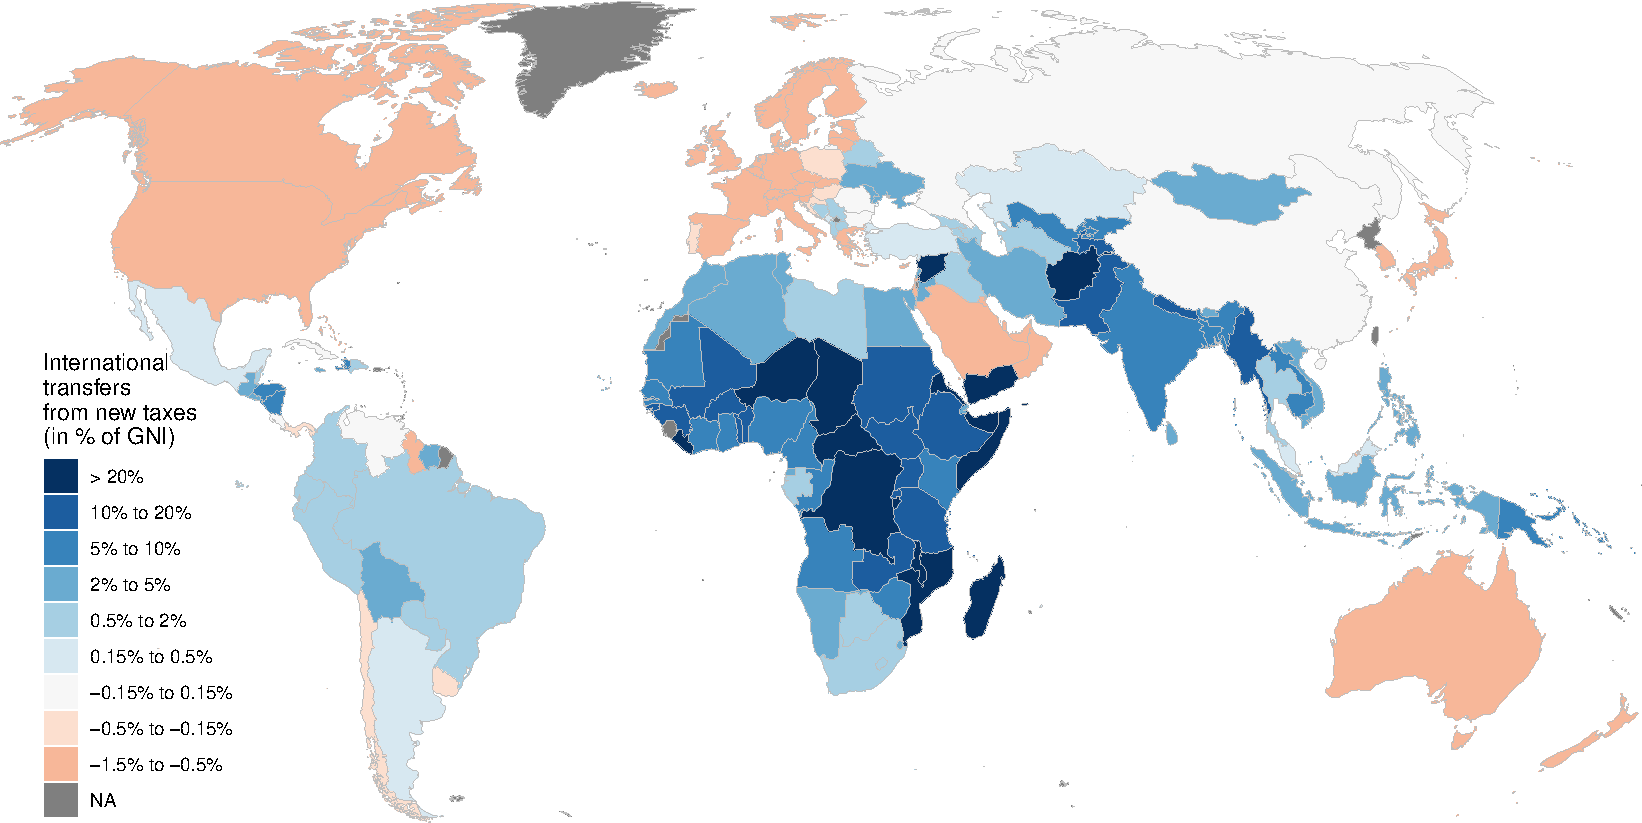
\includegraphics[width=1\textwidth]{net_gain_over_gdp_both_taxes_pop.pdf}} 
\end{figure}

\begin{figure}[h!] 
    \caption{Net gain for state budgets from new taxes and international transfers (revenue plus net transfer). \textit{All countries' governments gain. }}\label{fig:budget_gain_both_taxes}
    \makebox[\textwidth][c]{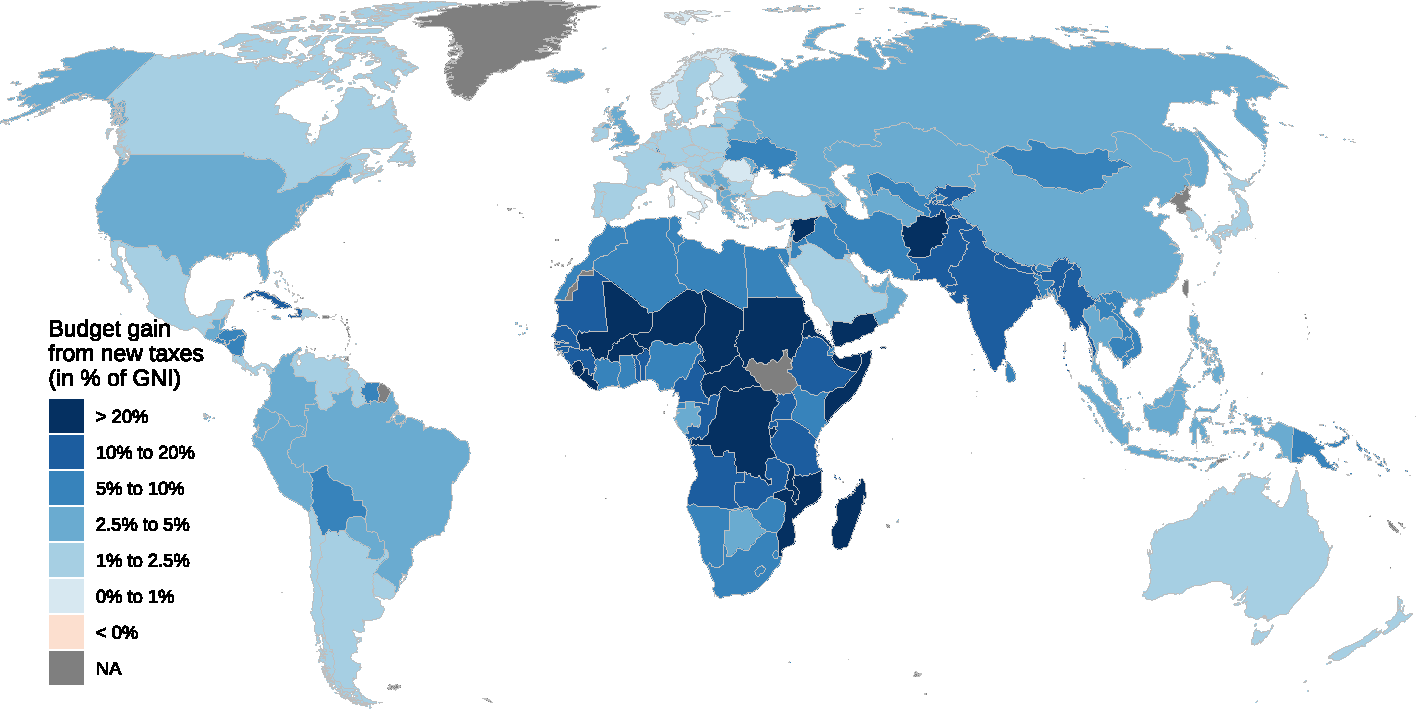
\includegraphics[width=.95\textwidth]{budget_gain_over_gdp_both_taxes_pop.pdf}} 
\end{figure}

\section{Proposal for an International Treaty}
The group of countries forming what could be called the Sustainable Union would have to agree on a number of elements: (i) a target for revenues from new levies on the richest and on pollution, say at least 2\% of their GNI; (ii) a common contribution to sustainable development, that we propose at 1\% of GNI; and (iii) a global carbon budget, say 1,000~GtCO$_\text{2}$ starting in 2025.
The parties to the Union would be expected to apply minimum rates of taxation on CO$_\text{2}$ emissions, individual wealth, and financial transactions, and to create a global asset register to list the assets held by each person. Tax avoidance would be prevented thanks to the extraterritorial mechanism of the ``tax collector of last resort'' proposed by the economist Gabriel \cite{zucman_blueprint_2024}. The Union would collect the ``missing'' tax due to the non-application by countries outside the Union of the minimum rates on multinational profits and individual wealth. In this case, the Union would demand payment of the “missing” tax, pro rata to the activities of the company (or companies controlled by the wealthy individual) that take place inside the Union, on pain of retaliatory measures against the company in question. These revenues would be used to increase transfers from the Union to the countries of the Global South.  

To respect the plurality of solutions and the sovereignty of States, the treaty would leave the choice of programs to be financed to the beneficiary States, provided they are validated by a multilateral agency. The agency in question would ensure that funds are traceable, and that they finance only public services, social protection and sustainable infrastructure. In the event of non-compliance with conditionalities, management of the funds would be entrusted to (another) multilateral agency, which would ensure that the population benefits. This mechanism would guarantee that transfers contribute to the intended uses and that they are not diverted nor misused.

\section{A Pragmatic Treaty in the Interest of the Greatest Number}
The Union would be open to all countries. To encourage as many countries as possible to join, the treaty could include elements of flexibility and conditional cooperation. In particular, the participation required of a high-income country could be reduced to the extent that other high-income countries did not participate. Thus, if the European countries join the Union but the United States and Japan do not, Europe's contribution could be halved. Also, to facilitate the accession to the Union of fossil-dependent countries such as China, Iran or Mongolia, a country could make its participation in carbon pricing conditional on an exemption from the system of taxes and transfers (it would then be subject to the same carbon price as the others but would neither be a beneficiary nor a contributor of transfers), provided this is accepted by the majority of other countries (weighted by their population). Finally, a country could make its participation conditional on the participation of one or more other countries, or on the GNI or emissions covered by the Union exceeding a threshold. For example, the European Union could choose to participate on condition that 60\% of global emissions are covered, which would de facto make its participation conditional on that of China (which accounts for 30\% of global emissions).

Various countries in the Global South could spearhead such a Union. The African Union has already taken similar positions \citep{african_union_african_2023}. Brazil is hosting the next COP of the UNFCCC. Mexico is presided over by a lead author of the fifth IPCC report. India would have strong interest to join such a Union, since it would receive large transfers from the rest of the world. China, with a per capita income equal to the world average, would be neither a contributor nor a beneficiary. It would have an interest in participating to ensure a low-carbon future in the long term, and outlets for its low-carbon equipment exports in the short term. We do not expect high-income fossil fuel exporters such as the United States, Russia, or Saudi Arabia to participate in the Union in the short term (though Democratic U.S. States such as California or New York could join it). Nonetheless, a Union composed of the Global South, China, the European Union, and some other high-income countries (Japan, South Korea, the UK, Canada…) would already cover 72\% of global CO$_\text{2}$ emissions. If such a Union respects an emissions pathway compatible with a global warming of +1.8\textdegree{}C in 2100, and assuming that non-participating countries follow a business-as-usual scenario without additional climate policies, global warming would reach +2.0\textdegree{}C in 2100, that is 0.6\textdegree{}C less than if the whole world follows the business-as-usual scenario [Anonymized for the review].%\citep{fabre_global_2025}.

\section{Societal Support for the Treaty}
Many people believe that such a treaty is politically impossible, especially in high-income countries. Yet recent academic surveys reveal strong public support for international climate policies, supranational governance and North-to-South solidarity. A survey of 125 countries shows that 69\% of people are willing to contribute 1\% of their income to fight climate change \citep{andre_globally_2024}. Another one in 17 countries (which include China, India, Russia, France, and Egypt) reveals that around 70\% of the population support a global democratic government to deal with global issues \citep{ghassim_who_2024}. A last survey shows that a global tax on millionaires to fund low-income countries is supported by 8 out of 10 people in high-income countries, that three quarters of Europeans and a majority of Americans support the internationally redistributive carbon pricing outlined above, and that parties advocating global redistribution could win votes in elections \citep{fabre_majority_2025}. Admittedly, despite public support, the prospect of global cooperation on sustainable development and climate action is dim in the short term, due to other political constraints, including hostile governments in major countries like the U.S. However, the direction of world politics could well shift in a few years, and a coalition of the willing could make progress despite the opposition of major countries, particularly on the preparatory work required for such an ambitious proposal. 

\section{A Solution Based on Climate Justice}
Since the start of the climate negotiations in 1992, the countries of the Global South have been demanding a financial contribution from the countries of the Global North, in recognition of their overriding responsibility for climate change, and to finance their sustainable development. The proposed Union would respect this legitimate demand. It would set a benchmark for contributions and transfers, resolving a long-standing debate on the distribution of decarbonization efforts. Financial contributions would be proportional to GNI, while financial transfers and emission rights would be proportional to the size of the population in each country. In this way, countries with per capita incomes below the global average would benefit financially (see Figure \ref{fig:gain_both_taxes}). Countries with per capita incomes above the world average would be net contributors, but the new taxes would be paid by the richest individuals, generating additional resources for their governments. Such a treaty could garner wide support, since the population of each country would benefit from a more stable climate, increased public revenues, and sustainable development.

Although they still need to be amended and negotiated, we believe that the principles and instruments that we put forward can pave the way for fruitful international agreements. Public attitudes suggest that high-level political impetus, prepared by extensive legal and diplomatic work, could make this vision for sustainable development a reality. We hope that our proposals can contribute to a positive political tipping point where a much larger and growing group of nations work together to solve humanity's great challenges.

\clearpage
\paragraph{Conflict of interest.} We have no conflict of interest to declare.

% \paragraph{Acknowledgements} % TODO

\renewcommand{\url}[1]{\href{#1}{Link}} % NCCcomment
% \bibliographystyle{plainnaturl_clean} % NCCcomment
% \bibliography{global_tax_attitudes}
% \clearpage
\begin{thebibliography}{9}
\providecommand{\natexlab}[1]{#1}
\providecommand{\url}[1]{\texttt{#1}}
\expandafter\ifx\csname urlstyle\endcsname\relax
  \providecommand{\doi}[1]{doi: #1}\else
  \providecommand{\doi}{doi: \begingroup \urlstyle{rm}\Url}\fi

\bibitem[Acemoglu \& Johnson(2024)]{acemoglu_urgent_2024}
D.~Acemoglu \& S.~Johnson.
\newblock The {{Urgent Need}} to {{Tax Digital Advertising}}.
\newblock 2024.
\newblock
  \url{https://shapingwork.mit.edu/wp-content/uploads/2024/04/Digital-Ad-Tax\_Policy-Brief.pdf}.

\bibitem[African~Union(2023)]{african_union_african_2023}
.~African~Union.
\newblock The {{African Leaders Nairobi Declaration}} on {{Climate Change}} and
  {{Call}} to {{Action}}.
\newblock Technical report, 2023.
\newblock
  \url{https://media.africaclimatesummit.org/NAIROBI+Declaration+FURTHER+edited+060923+EN+920AM.pdf}.

\bibitem[Andre et~al.(2024)Andre, Boneva, Chopra, \& Falk]{andre_globally_2024}
P.~Andre, T.~Boneva, F.~Chopra, \& A.~Falk.
\newblock Globally representative evidence on the actual and perceived support
  for climate action.
\newblock \emph{Nature Climate Change}, 2024.
\newblock \url{https://www.nature.com/articles/s41558-024-01925-3}.

\bibitem[Bolton et~al.(2025)Bolton, Edenhofer, Kleinnijenhuis, Rockstr{\"o}m,
  \& Zettelmeyer]{bolton_why_2025}
P.~Bolton, O.~Edenhofer, A.~Kleinnijenhuis, J.~Rockstr{\"o}m, \&
  J.~Zettelmeyer.
\newblock Why coalitions of wealthy nations should fund others to decarbonize.
\newblock \emph{Nature}, 2025.
\newblock \url{https://www.nature.com/articles/d41586-025-00779-9}.

\bibitem[Fabre et~al.(2025)Fabre, Douenne, \& Mattauch]{fabre_majority_2025}
A.~Fabre, T.~Douenne, \& L.~Mattauch.
\newblock Majority support for global redistributive and climate policies.
\newblock \emph{Nature Human Behaviour}, 2025.
\newblock \url{https://www.nature.com/articles/s41562-025-02175-9}.

\bibitem[Ghassim \& Pauli(2024)]{ghassim_who_2024}
F.~Ghassim \& M.~Pauli.
\newblock Who on {{Earth Wants}} a {{World Government}}, {{What Kind}}, and
  {{Why}}? {{An International Survey Experiment}}.
\newblock \emph{International Studies Quarterly}, 2024.
\newblock \url{https://doi.org/10.1093/isq/sqae105}.

\bibitem[Hourcade et~al.(2025)Hourcade, Dasgupta, De~Coninck, Glemarec, Grubb,
  Kainuma, La~Rovere, Vallejo, Murasawa, Netto~Schneider, Sokona, \&
  Winkler]{hourcade_climate_2025}
J.~C. Hourcade, D.~Dasgupta, H.~De~Coninck, Y.~Glemarec, M.~Grubb, M.~Kainuma,
  E.~La~Rovere, L.~Vallejo, L.~Murasawa, M.~Netto~Schneider, Y.~Sokona, \&
  H.~Winkler.
\newblock A {{Climate Finance Initiative}} at {{COP30}}: {{A Multisovereign
  Guarantee Mechanism}} for {{Accelerated Climate Investments}} in {{Developing
  Countries}}.
\newblock 2025.
\newblock
  \url{https://unfccc.int/sites/default/files/resource/Centro\_Clima\_Baku\_to\_Bel\%C3\%A9m\_Roadmap.pdf}.

\bibitem[{Pisani-Ferry} et~al.(2025){Pisani-Ferry}, {di Mauro}, \&
  Zettelmeyer]{pisani-ferry_global_2025}
E.~J. {Pisani-Ferry}, B.~W. {di Mauro}, \& J.~Zettelmeyer.
\newblock Global action without global governance.
\newblock \emph{CEPR}, 2025.
\newblock
  \url{https://cepr.org/publications/books-and-reports/paris-report-3-global-action-without-global-governance-building}.

\bibitem[Zucman(2024)]{zucman_blueprint_2024}
G.~Zucman.
\newblock A blueprint for a coordinated minimum effective taxation standard for
  ultra-high-net-worth individuals.
\newblock 2024.
\newblock
  \url{https://www.taxobservatory.eu/publication/a-blueprint-for-a-coordinated-minimum-effective-taxation-standard-for-ultra-high-net-worth-individuals/}.

\end{thebibliography}

\end{bibunit}
\begin{bibunit}

\appendix
\clearpage
\section{Appendix}

% \section{Summary}\label{sec:intro}
% \begin{abstract}
  We estimate the revenues by country from six global taxes: a tax on wealth above \$100 million, a small carbon tax, a higher minimum corporate income tax, % carbon tax is the only one whose transfers are based on GDP
  a financial transaction tax, a tax on maritime fuel and one on aviation fuel (Table \ref{tab:transfers_gain}). \$2.1 trillion would be collected. % (2\% of the world GDP). 
  %
  We further estimate international transfers that could be financed.  %according to the proposed allocation of revenues between countries. 
  Namely, we reallocate 1\% of each country's GNI to all countries in proportion to their %adult 
  population, and one half of the wealth tax to countries with a per capita GNI lower than twice the world average, in proportion to their distance to this threshold. The combination of these taxes and transfers entail \$766 billion in North--South transfers.  
% \end{abstract}


\subsection{Wealth tax}\label{sec:wealth}

% Under its G20 presidency, Brazil commissionned a report on a global tax on ultra-high wealth. Indeed, the richest pay less taxes than average people in proportion to their contributive capacity, as most of their income is in the form of unrealized capital gains not subject to taxation. The report by \cite{zucman_blueprint_2024} proposes a top-up tax on the wealth of individual owning more than \$100 million, to collect the missing income tax revenue. With a 3\% top-up tax, a billionaire who already pays taxes amounting to 1\% of its wealth would be liable to an additional 2\% tax. Although a top-up tax may be 

We simulate two wealth taxes. First, a global tax on ultra-high wealth: a 3\% tax on all individual wealth in excess of \$100 million. Second, a national wealth tax: a 2\% tax on wealth in excess of \$5 million. These taxes add up,\footnote{For example, with a wealth of \$150 million, someone would pay each year a tax of 2.9\% on their wealth: 1\% from the tax on ultra-high wealth ($3\% \cdot \left(150-100\right)=1.5M$) and 1.9\% from the national wealth tax.% ($2\% \cdot \left(150-5\right)=2.9M$).
} so the highest marginal tax rate is 5\%.


The World Inequality Lab offers an \href{https://wid.world/world-wealth-tax-simulator/}{online simulator} to estimate the revenue collected by a custom wealth tax in each world region. Building on this work, we disaggregate the revenue estimates at the country level. Courtesy of Félix Bajard, we obtained the simulator's underlying data for 50 countries covering 95\% of global wealth tax revenue. To impute missing data, we predict the taxable base from a linear regression of the log of taxable base on the log of nominal GDP per capita, weighted by country population. 

Following \cite{zucman_blueprint_2024}, we assume 20\% of tax evasion. We also conservatively assume that asset prices would decline by 10\%. Half of the revenue from the global tax on ultra-high wealth would not be retained domestically but channeled into a fund to finance sustainable development. This fund would return revenues to countries with a per capita GNI below a threshold. We fix this eligibility threshold at twice the world average per capita GNI, or \$26,885 per year (in nominal terms). Finally, eligible countries receive a transfer per person %adult 
proportional to the difference between the threshold and their GNI per capita.

% \clearpage
\begin{table}[!h]
  \caption{\label{tab:transfers_gain}Global taxes: international transfers, budget gain, revenues collected (\% of GNI). }
  \makebox[\textwidth][c]{
  
\begin{tabular}[t]{lccccccccc}
\toprule
  & \makecell{Int'l\\transfers} & \makecell{Budget\\gain} & \makecell{Wealth\\Tax (3\%\\$>$100M)} & \makecell{Wealth\\Tax (2\%\\$>$5M)} & \makecell{Financ.\\Transac.\\Tax} & \makecell{Carbon\\Tax\\(10\$/t)} & \makecell{Maritime\\fuel tax\\(100\$/t)} & \makecell{Aviation\\fuel tax\\(300\$/t)} & \makecell{Corporate\\inc. tax\\(min 21\%)}\\
\midrule
World & 0.0 & 3.2 & 0.72 & 1.28 & 0.32 & 0.33 & 0.10 & 0.22 & 0.28\\
Afghanistan & 43.4 & 46.1 & 0.29 & 0.49 & 0.58 & 0.88 & 0.01 & 0.42 & 0.00\\
DRC & 21.7 & 23.0 & 0.32 & 0.55 & 0.13 & 0.10 & 0.11 & 0.10 & 0.00\\
Myanmar & 16.2 & 18.3 & 0.36 & 0.61 & 0.51 & 0.35 & 0.04 & 0.25 & 0.00\\
Sudan & 15.6 & 17.7 & 0.34 & 0.59 & 0.40 & 0.47 & 0.05 & 0.32 & 0.00\\
Uganda & 14.6 & 16.2 & 0.34 & 0.59 & 0.20 & 0.15 & 0.01 & 0.33 & 0.00\\
Ethiopia & 13.7 & 15.4 & 0.35 & 0.60 & 0.14 & 0.12 & 0.00 & 0.45 & 0.00\\
Tanzania & 11.9 & 13.5 & 0.36 & 0.61 & 0.22 & 0.20 & 0.02 & 0.26 & 0.00\\
Pakistan & 10.7 & 11.9 & 0.02 & 0.05 & 0.35 & 0.49 & 0.04 & 0.18 & 0.00\\
Nigeria & 7.1 & 8.8 & 0.10 & 0.62 & 0.24 & 0.34 & 0.35 & 0.09 & 0.00\\
Kenya & 6.9 & 8.7 & 0.39 & 0.67 & 0.15 & 0.18 & 0.02 & 0.42 & 0.00\\
India & 6.4 & 10.3 & 1.26 & 1.51 & 0.26 & 0.61 & 0.05 & 0.17 & 0.01\\
Bangladesh & 6.0 & 6.5 & 0.03 & 0.06 & 0.13 & 0.17 & 0.02 & 0.08 & 0.00\\
Morocco & 4.1 & 6.7 & 0.44 & 0.74 & 0.23 & 0.49 & 0.18 & 0.46 & 0.00\\
Vietnam & 4.0 & 5.7 & 0.01 & 0.56 & 0.17 & 0.50 & 0.11 & 0.41 & 0.00\\
Egypt & 3.4 & 5.5 & 0.44 & 0.47 & 0.29 & 0.63 & 0.07 & 0.20 & 0.00\\
Philippines & 3.3 & 4.8 & 0.28 & 0.49 & 0.19 & 0.22 & 0.03 & 0.37 & 0.00\\
Ukraine & 3.2 & 6.1 & 0.46 & 0.78 & 0.21 & 0.98 & 0.30 & 0.19 & 0.00\\
Iran & 3.1 & 7.0 & 0.45 & 0.77 & 0.37 & 1.63 & 0.39 & 0.22 & 0.00\\
Indonesia & 2.9 & 4.9 & 0.25 & 0.41 & 0.23 & 0.45 & 0.23 & 0.32 & 0.04\\
Algeria & 2.5 & 5.1 & 0.46 & 0.78 & 0.26 & 0.72 & 0.18 & 0.14 & 0.00\\
Thailand & 1.8 & 4.9 & 0.49 & 0.83 & 0.25 & 0.61 & 0.20 & 0.79 & 0.00\\
Colombia & 1.7 & 4.1 & 0.49 & 0.83 & 0.20 & 0.24 & 0.36 & 0.30 & 0.00\\
Iraq & 1.7 & 5.7 & 0.47 & 0.80 & 0.33 & 1.00 & 1.34 & 0.09 & 0.00\\
South Africa & 1.6 & 5.6 & 0.33 & 0.64 & 0.19 & 1.12 & 0.53 & 0.38 & 0.83\\
Brazil & 0.9 & 3.8 & 0.60 & 0.78 & 0.17 & 0.29 & 0.57 & 0.23 & 0.24\\
Turkey & 0.5 & 2.0 & 0.13 & 0.23 & 0.24 & 0.45 & 0.10 & 0.37 & 0.00\\
Mexico & 0.2 & 2.3 & 0.59 & 0.73 & 0.17 & 0.30 & 0.05 & 0.22 & 0.03\\
Argentina & 0.2 & 2.6 & 0.54 & 0.92 & 0.15 & 0.35 & 0.18 & 0.23 & 0.01\\
China & -0.1 & 3.5 & 1.06 & 1.51 & 0.10 & 0.58 & 0.05 & 0.15 & 0.12\\
Russia & -0.1 & 3.2 & 0.87 & 1.06 & 0.18 & 0.79 & 0.16 & 0.24 & 0.00\\
Poland & -0.2 & 1.5 & 0.11 & 0.19 & 0.16 & 0.44 & 0.07 & 0.10 & 0.59\\
Saudi Arabia & -0.6 & 1.4 & 0.11 & 0.40 & 0.15 & 0.59 & 0.52 & 0.25 & 0.00\\
Spain & -0.6 & 1.1 & 0.24 & 0.40 & 0.22 & 0.14 & 0.06 & 0.37 & 0.34\\
Japan & -0.7 & 1.2 & 0.22 & 0.54 & 0.40 & 0.23 & 0.05 & 0.14 & 0.28\\
South Korea & -0.7 & 1.3 & 0.31 & 0.53 & 0.11 & 0.30 & 0.16 & 0.20 & 0.38\\
Italy & -0.8 & 0.8 & 0.35 & 0.50 & 0.17 & 0.13 & 0.04 & 0.15 & 0.22\\
United Kingdom & -0.8 & 3.2 & 0.25 & 0.43 & 2.36 & 0.12 & 0.04 & 0.28 & 0.55\\
Germany & -1.0 & 1.6 & 0.50 & 1.00 & 0.22 & 0.16 & 0.06 & 0.15 & 0.44\\
Canada & -1.0 & 2.4 & 0.59 & 1.25 & 0.09 & 0.27 & 0.08 & 0.26 & 0.92\\
France & -1.1 & 2.3 & 0.80 & 1.57 & 0.33 & 0.10 & 0.02 & 0.20 & 0.40\\
United States & -1.3 & 2.6 & 0.90 & 1.92 & 0.27 & 0.19 & 0.03 & 0.21 & 0.34\\
\bottomrule
\end{tabular}
} 
{\footnotesize \textit{Note:}  Budget gain denotes the sum of all other columns: international transfer and revenues collected. %revenue collected (last six columns) plus (net) international transfer (first column).
}
\end{table}
% \clearpage

\begin{table}[!h]
  \vspace{-1cm}
  \caption{\label{tab:transfers_balance}Comparison of population vs. adult pop. entitlement; carbon balance (\% of GNI). }
  \makebox[\textwidth][c]{
  
\begin{tabular}[t]{lcccccc}
\toprule
  & \makecell{Int'l\\transfers\\(population)} & \makecell{Int'l\\transfers\\(adult)} & \makecell{Budget\\gain\\(population)} & \makecell{Budget\\gain\\(adult)} & \makecell{Annualized\\carbon balance\\1850-2024} & \makecell{Annualized\\carbon balance\\1990-2024}\\
\midrule
Afghanistan & 47.6 & 43.4 & 50.3 & 46.1 & 264.9 & 166.2\\
DRC & 24.4 & 21.7 & 25.7 & 23.0 & 139.5 & 95.2\\
Sudan & 16.8 & 15.6 & 19.0 & 17.7 & 96.2 & 65.3\\
Uganda & 16.3 & 14.6 & 17.9 & 16.2 & 87.0 & 61.4\\
Myanmar & 15.8 & 16.2 & 18.0 & 18.3 & 130.2 & 69.9\\
Ethiopia & 14.7 & 13.7 & 16.4 & 15.4 & 88.0 & 58.1\\
Tanzania & 13.1 & 11.9 & 14.8 & 13.5 & 75.1 & 52.0\\
Pakistan & 11.3 & 10.7 & 12.4 & 11.9 & 60.9 & 39.3\\
Nigeria & 7.8 & 7.1 & 9.6 & 8.8 & 47.4 & 30.1\\
Kenya & 7.3 & 6.9 & 9.2 & 8.7 & 42.3 & 30.1\\
India & 6.3 & 6.4 & 10.2 & 10.3 & 43.3 & 22.7\\
Bangladesh & 5.9 & 6.0 & 6.4 & 6.5 & 44.5 & 26.2\\
Morocco & 4.1 & 4.1 & 6.6 & 6.7 & 30.0 & 15.2\\
Vietnam & 3.8 & 4.0 & 5.6 & 5.7 & 27.6 & 14.0\\
Egypt & 3.5 & 3.4 & 5.6 & 5.5 & 19.1 & 10.0\\
Philippines & 3.3 & 3.3 & 4.9 & 4.8 & 22.5 & 14.2\\
Iran & 3.0 & 3.1 & 6.9 & 7.0 & -6.0 & -9.6\\
Ukraine & 3.0 & 3.2 & 5.9 & 6.1 & -47.4 & -13.9\\
Indonesia & 2.9 & 2.9 & 4.8 & 4.9 & 20.0 & 9.9\\
Algeria & 2.5 & 2.5 & 5.1 & 5.1 & 10.3 & 3.9\\
Iraq & 1.8 & 1.7 & 5.9 & 5.7 & 2.5 & 0.1\\
Thailand & 1.6 & 1.8 & 4.8 & 4.9 & 10.1 & 1.9\\
Colombia & 1.6 & 1.7 & 4.0 & 4.1 & 13.2 & 7.7\\
South Africa & 1.6 & 1.6 & 5.6 & 5.6 & -17.3 & -10.3\\
Brazil & 0.8 & 0.9 & 3.7 & 3.8 & 9.4 & 4.7\\
Turkey & 0.5 & 0.5 & 2.0 & 2.0 & 3.6 & 0.3\\
Mexico & 0.2 & 0.2 & 2.2 & 2.3 & 1.2 & 0.5\\
Argentina & 0.2 & 0.2 & 2.5 & 2.6 & 1.9 & 0.3\\
China & -0.1 & -0.1 & 3.4 & 3.5 & 3.8 & -1.3\\
Russia & -0.1 & -0.1 & 3.1 & 3.2 & -22.9 & -11.5\\
Poland & -0.2 & -0.2 & 1.5 & 1.5 & -13.7 & -5.2\\
Saudi Arabia & -0.6 & -0.6 & 1.4 & 1.4 & -6.2 & -5.6\\
Spain & -0.6 & -0.6 & 1.1 & 1.1 & -0.5 & -1.2\\
Japan & -0.7 & -0.7 & 1.2 & 1.2 & -3.9 & -3.1\\
South Korea & -0.7 & -0.7 & 1.3 & 1.3 & -2.5 & -3.7\\
Italy & -0.8 & -0.8 & 0.8 & 0.8 & -1.3 & -1.5\\
United Kingdom & -0.8 & -0.8 & 3.2 & 3.2 & -10.5 & -1.6\\
Germany & -1.0 & -1.0 & 1.6 & 1.6 & -9.6 & -2.6\\
Canada & -1.0 & -1.0 & 2.4 & 2.4 & -7.9 & -4.3\\
France & -1.1 & -1.1 & 2.3 & 2.3 & -3.5 & -0.7\\
United States & -1.3 & -1.3 & 2.6 & 2.6 & -9.2 & -3.5\\
\bottomrule
\end{tabular}
} 
{\footnotesize \textit{Note:} Budget gain denotes the country net entitlements, i.e. the revenue it collects plus the net international transfer. International transfers denotes the country net entitlements minus taxes paid in the country. The carbon balance is separated from the tax proposals, it corresponds to the carbon credit or debt over 1850--2024 (or 1990--2024), priced at \$185/tCO$_\text{2}$ and annualized at 3.5\%. For example, a country with excess emissions compared to the world average accumulates a carbon debt. % Budget gain denotes the sum of all other columns: international transfer and revenues collected. %revenue collected (last six columns) plus (net) international transfer (first column).
}
\end{table}
% \clearpage


\subsection{Financial Transactions Tax}\label{sec:ftt}

\cite{pekanov_global_2019} estimate the revenues from a Financial Transactions Tax (FTT). Following the proposal by the European Commission (2011), they use a rate of 0.1\% of bonds and stocks and a rate of 0.01\% on derivatives. We use their baseline scenario, which assumes evasion rates of 15\% on bonds and stocks and 70\% on derivatives, together with an elasticity of trading volumes of $-$1.\footnote{The formula is: $\text{Revenue} = \text{tax rate} \cdot \text{volume} \cdot \text{evasion} \cdot \left(1 + \text{tax rate} / \text{transaction cost}\right)^\text{elasticity}$.} 

\cite{pekanov_global_2019} provide estimates at the global level and for 18 high-income countries. We allocate the global revenue that does not originate from these 18 countries to remaining countries, in proportion to their GDP. 22\% of world revenues would be collected in these remaining countries, with a revenue amounting to 0.1\% of their GDP (vs. 0.56\% of GDP for the 18 high-income countries).
% In these remaining countries, the FTT collects 22\% of the world total, and 0.1\% of these countries' GDP (vs. 0.56\% of GDP in the 18 high-income countries).


\subsection{Carbon price}\label{sec:carbon}

We model simulate the international transfers a \$100/tCO$_\text{2}$ carbon price applied to all non-LULUCF CO$_\text{2}$ emissions. At the global level, and neglecting behavioral responses, 0.33\% of the world nominal GDP would be collected. 
%Contrary to the other taxes studied here, the revenues of the carbon price are not entirely pooled at the global level. Instead, we assume that 0.2\% of each country's nominal GDP would be pooled and rebated to all countries in proportion to their adult population. With some exceptions (such as Ireland and Switzerland), the carbon price revenues would cover more than the transfer owed to the rest of the world, leaving revenues for domestic spending even in high-income countries.

\subsection{Maritime fuel levy}\label{sec:wealth}

We simulate the revenues of a \$100/tCO$_\text{2}$ levy on maritime fuel. The emissions from shipping by country are given by the simple average between the minimum and maximum estimates of \citet{dequiedt_navigating_2024}, who graciously provided the data. 

\subsection{Aviation fuel levy}\label{sec:wealth}

Using data from \cite{graver_CO2_2018},\footnote{We use the data unadjusted for tourism.} we estimate the revenues from a tax on all flights (domestic and international). Due to complex climate effects such as contrails, aviation the global warming potential of aviation (GWP*$_\text{100}$) is 3 times the warming caused by its CO$_\text{2}$ emissions \citep{lee_contribution_2021}. To fully account for all effects on global warming, the carbon levy on aviation should be multiplied by that factor. Therefore, we simulate a \$300/tCO$_\text{2}$ tax on aviation fuel, comparable to the \$100/tCO$_\text{2}$ tax on maritime fuel. We use the 2018 data without adjusting for the expected increase in air traffic, and without adjusting for the decrease in traffic that would follow the tax.\footnote{More generally, we do not adjust for inflation or changes in volumes throughout this technical note. Figures are only provided to get ballpark estimates and cannot be very precise.}

\subsection{Higher minimum corporate income tax}

We estimate extra revenue by country if the internationally agreed minimum rate on corporate income tax was raised from 15\% to 21\%, with no carve-out. We use data from the \href{https://www.taxobservatory.eu/fr/base-de-donn%C3%A9es/the-tax-deficit-simulator/}{tax deficit simulator} from the EU Tax Observatory. These estimates are available for 45 countries (from OECD and the G20). We impute missing data only for three high-income countries (Iceland, Israel, New Zealand) and conservatively assume no extra revenue for other (developing) countries with missing data.

\subsection{Carbon balance}

On top of the proposed new taxes, we compute historical responsibilites for climate change. We define a carbon balance as the sum of a country's excess emissions compared to the world average, each year between 1850 and 2024, priced at $p=$ \$185/tCO$_\text{2}$ (which corresponds to the social cost of carbon according to \citealp{rennert_comprehensive_2022}). 
% We report the carbon balance over nominal GNI in 2025 country-by-country in Table \ref{tab:transfers_balance}.
In Table \ref{tab:transfers_balance}, we report the carbon balance annualized at a risk-adjusted discount rate of $r =$ 3.5\%. Denoting $e_t^c$ the emissions of country $c$ in year $t$, and $\pi_t^c$ its share of the world population at $t$, its annualized carbon balance over nominal GNI, $B_c$, is: $ B_c = r \cdot p \cdot \sum_{t=1850}^{2024} e_t^c - \pi_t^c \cdot \sum_c e_t^c / \text{GNI}_c^{2023}\text{.}$ Our computations are based on historical CO$_\text{2}$ emissions excluding LULUCF sector \citep{gutschow_country-resolved_2021}.

\clearpage
\renewcommand{\url}[1]{\href{#1}{Link}} 

\begin{thebibliography}{7}
\providecommand{\natexlab}[1]{#1}
\providecommand{\url}[1]{\texttt{#1}}
\expandafter\ifx\csname urlstyle\endcsname\relax
  \providecommand{\doi}[1]{doi: #1}\else
  \providecommand{\doi}{doi: \begingroup \urlstyle{rm}\Url}\fi

\bibitem[Dequiedt et~al.(2024)Dequiedt, De~Ubeda, \&
  Mien]{dequiedt_navigating_2024}
V.~Dequiedt, A.-A. De~Ubeda, \& {\'E}.~Mien.
\newblock Navigating international taxation: {{The}} effects of a carbon levy
  on shipping.
\newblock 2024.
\newblock \url{https://hal.science/hal-04573868}.

\bibitem[Graver et~al.(2018)Graver, Zhang, \& Rutherford]{graver_CO2_2018}
B.~Graver, K.~Zhang, \& D.~Rutherford.
\newblock {{CO2}} emissions from commercial aviation, 2018.
\newblock 2018.

\bibitem[G{\"u}tschow et~al.(2021)G{\"u}tschow, Jeffery, G{\"u}nther, \&
  Meinshausen]{gutschow_country-resolved_2021}
J.~G{\"u}tschow, M.~L. Jeffery, A.~G{\"u}nther, \& M.~Meinshausen.
\newblock Country-resolved combined emission and socio-economic pathways based
  on the {{Representative Concentration Pathway}} ({{RCP}}) and {{Shared
  Socio-Economic Pathway}} ({{SSP}}) scenarios.
\newblock \emph{Earth System Science Data}, 2021.
\newblock \url{https://essd.copernicus.org/articles/13/1005/2021/}.

\bibitem[Lee et~al.(2021)Lee, Fahey, Skowron, Allen, Burkhardt, Chen, Doherty,
  Freeman, Forster, Fuglestvedt, Gettelman, De~Le{\'o}n, Lim, Lund, Millar,
  Owen, Penner, Pitari, Prather, Sausen, \& Wilcox]{lee_contribution_2021}
D.~S. Lee, D.~W. Fahey, A.~Skowron, M.~R. Allen, U.~Burkhardt, Q.~Chen, S.~J.
  Doherty, S.~Freeman, P.~M. Forster, J.~Fuglestvedt, A.~Gettelman, R.~R.
  De~Le{\'o}n, L.~L. Lim, M.~T. Lund, R.~J. Millar, B.~Owen, J.~E. Penner,
  G.~Pitari, M.~J. Prather, R.~Sausen, \& L.~J. Wilcox.
\newblock The contribution of global aviation to anthropogenic climate forcing
  for 2000 to 2018.
\newblock \emph{Atmospheric Environment}, 2021.
\newblock
  \url{https://www.sciencedirect.com/science/article/pii/S1352231020305689}.

\bibitem[Pekanov \& Schratzenstaller(2019)]{pekanov_global_2019}
A.~Pekanov \& M.~Schratzenstaller.
\newblock A {{Global Financial Transaction Tax}} - {{Theory}}, {{Practice}} and
  {{Potential Revenues}}, 2019.
\newblock \url{https://papers.ssrn.com/abstract=3407855}.

\bibitem[Rennert et~al.(2022)Rennert, Errickson, Prest, Rennels, Newell, Pizer,
  Kingdon, Wingenroth, Cooke, Parthum, Smith, Cromar, Diaz, Moore, M{\"u}ller,
  Plevin, Raftery, {\v S}ev{\v c}{\'i}kov{\'a}, Sheets, Stock, Tan, Watson,
  Wong, \& Anthoff]{rennert_comprehensive_2022}
K.~Rennert, F.~Errickson, B.~C. Prest, L.~Rennels, R.~G. Newell, W.~Pizer,
  C.~Kingdon, J.~Wingenroth, R.~Cooke, B.~Parthum, D.~Smith, K.~Cromar,
  D.~Diaz, F.~C. Moore, U.~K. M{\"u}ller, R.~J. Plevin, A.~E. Raftery, H.~{\v
  S}ev{\v c}{\'i}kov{\'a}, H.~Sheets, J.~H. Stock, T.~Tan, M.~Watson, T.~E.
  Wong, \& D.~Anthoff.
\newblock Comprehensive evidence implies a higher social cost of {{CO2}}.
\newblock \emph{Nature}, 2022.
\newblock \url{https://www.nature.com/articles/s41586-022-05224-9}.

\bibitem[Zucman(2024)]{zucman_blueprint_2024}
G.~Zucman.
\newblock A blueprint for a coordinated minimum effective taxation standard for
  ultra-high-net-worth individuals.
\newblock 2024.
\newblock
  \url{https://www.taxobservatory.eu/publication/a-blueprint-for-a-coordinated-minimum-effective-taxation-standard-for-ultra-high-net-worth-individuals/}.

\end{thebibliography}


\end{bibunit}
% \textit{Our figures are fully reproducible from our data and code, openly availably on\\ \href{https://github.com/bixiou/global_tax_attitudes/raw/main/code_global/new_taxes.R}{github.com/bixiou/global\_tax\_attitudes/raw/main/code\_global/main/raw/new\_taxes.R}. %We are here to feed the public debate on global redistribution. We welcome counter-proposals, criticisms and suggestions concerning (including pull requests).  
% }


% {\footnotesize
% \begingroup
% \setstretch{.5}
% \titleformat*{\section}{\fontsize{11pt}{14pt}\bfseries\selectfont}
% \renewcommand{\url}[1]{\href{#1}{Link}} % NCCcomment
% \renewcommand\bibname{\small Bibliography}
% \footnotesize
% \bibliographystyle{plainnaturl_clean} % NCCcomment
% \bibliography{global_tax_attitudes}
% \hphantom{\vphantom{
%     \begin{minipage}{\textwidth}
%         \bibliography{global_tax_attitudes}
%     \end{minipage}
% }}
% \endgroup }

\end{document}